\documentclass{article}

\usepackage[utf8]{inputenc}
\usepackage{graphicx} % Comandos para manejar imágenes
\graphicspath{ {./images/} } % Carpeta de imágenes

\setlength{\parskip}{2mm} % Espaciado

\usepackage[utf8]{inputenc}
\usepackage{geometry}
    \geometry{left=3cm,right=2cm,top=2cm,bottom=2cm}
%
\usepackage[spanish]{babel}
%
\usepackage[fixlanguage]{babelbib}
    \bibliographystyle{babunsrt}
%

\usepackage{floatrow}
\floatsetup[table]{style=plaintop}

\usepackage{url}

\usepackage[top=2cm, bottom=2.5cm, right=3 cm, left=3 cm]{geometry} % margenes

\usepackage{parskip} % Sangria

\title{Seminario cinco: Un modelo para predecir accidentes, comentarios sobre la presentación del Doctor Franco Basso}
\author{Cristóbal Galleguillos Ketterer$^{1}$\\
\small{$^{1}$Industrial PhD Program}\\
\small{Pontificia Universidad Católica de Valparaíso}\\
\small{cristobal.galleguillos@pucv.cl}
}
\date{\small{\today}}

\begin{document}

\maketitle

\section{Introducción}

Un accidente es un hecho de carácter fortuito, que generalmente provoca daños en la propiedad y en las personas. Los accidentes, dado su carácter no planificado, son imposibles de predecir, siendo, en la práctica, su control mediante estrategias preventivas.

En lo que respecta a seguridad vial, la accidentalidad posee un carácter crítico, ya que generalmente conllevan daños a la integridad de las personas, y otros efectos no deseados como daño a la propiedad y a la infraestructura vial.

La evolución de los accidentes y fallecidos en Chile se puede apreciar en el gráfico que se presenta en la Figura \ref{scc}, esta tendencia puede estar condicionada por diversas variable como el aumento del parque vehicular, las normas que regulan la velocidad, la tecnología de los vehículos u otras.

\begin{figure}[H]
\includegraphics[scale=0.5]{Images/acc.jpg}
\centering
\caption{Evolución siniestros de transito y fallecidos 1972-2019, Fuente CONACET}
\label{scc}
\end{figure}

El trabajo presentado por doctor Basso, nos muestra un modelo que permite predecir, en tiempo real, la ocurrencia de un accidente en una autopista urbana.

\subsection{Alcance}

La presentación de este trabajo no considera la revisión de la matemática presente en la metodología desarrollada por el doctor Basso, por estar fuera del alcance de las competencias del autor de este informe.

\section{Revisión de la literatura}

El profesor Basso, es un joven investigador, sus áreas de investigación son: Operations Research, Logistics and Transportation, Scheduling, Data Science y Crash Prediction. El trabajo presentado se basa en esta última área.

Como mencionó en su conferencia, en el área de Crash Prediction, es un campo relativamente nuevo en el área de la investigación aplicada en ingeniería, el autor pionero en esta línea es el profesor Abdel-Aty. La estructura conceptual de su investigación se puede ver en la Figura \ref{aty}.

\begin{figure}[H]
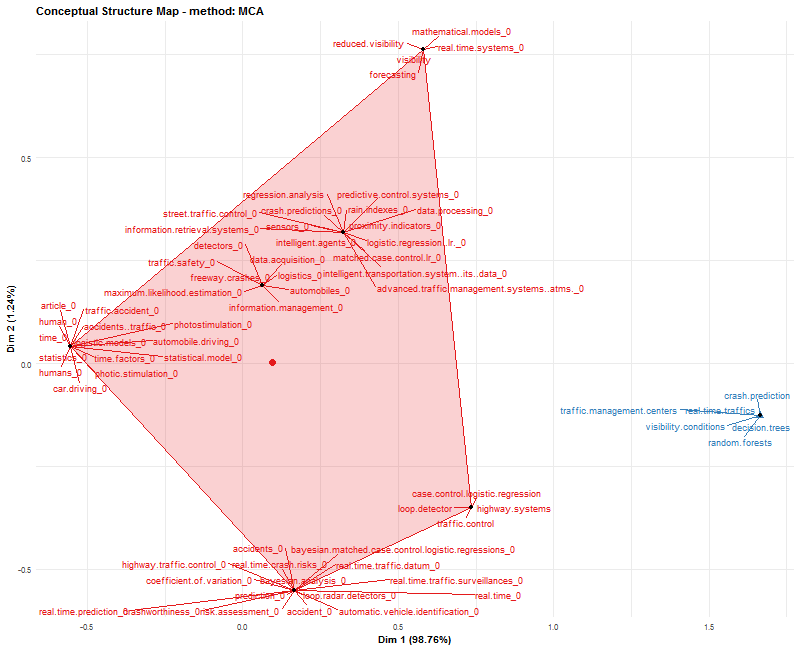
\includegraphics[scale=0.5]{Images/grafo.png}
\centering
\caption{Mapa de la estructura conceptual, profesor Abdel-Aty.}
\label{aty}
\end{figure}

Dentro del área de investigación de Crash Prediction, vemos una tasa de crecimiento en la producción científica de un 8,4\%, este crecimiento se ve reflejado en la Figura \ref{prod} (considerar que el año 2020 aún está  en curso)

\begin{figure}[H]
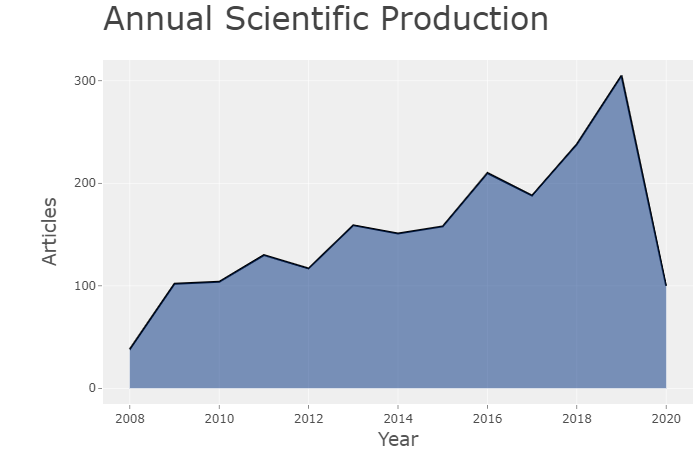
\includegraphics[scale=0.4]{Images/newplot (6).png}
\centering
\caption{Producción científica anual}
\label{prod}
\end{figure}

Finalmente presentamos la Figura \ref{arbol} donde vemos en el tronco central la relevancia de la investigación del profesor Abdel-Aty, en el campo de estudio de Crash Prediction.

\begin{figure}[H]
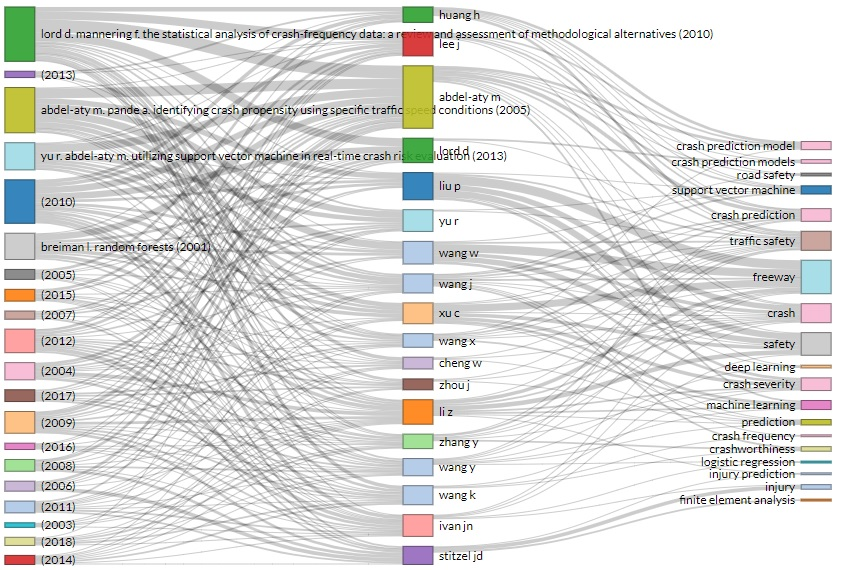
\includegraphics[scale=0.5]{Images/abdel.jpg}
\centering
\caption{Producción científica anual}
\label{arbol}
\end{figure}



\section{Marco teórico}

En la actualidad la adquisición de datos es cada vez mas frecuente en la industria, y con ello, se dispone de una gran cantidad de ellos, que ayudan en la toma de decisiones diarias, como en la operación de  una planta de packing o bien en la planificación del mantenimiento predictivo de una turbina.

Además, estos datos permiten establecer una historia de los procesos, y con posterioridad al uso operacional, quedan disponibles para su manejo y estudio.

Es de suponer que una gran cantidad de datos facilita el modelado de los procesos, sin embargo el problema radica en identificar los patrones de comportamiento y las variables relevantes dentro de estos grandes volúmenes de datos.

A esta técnica de manejo de datos se denomina \textit{Machine Learning}, las técnicas de \textit{Machine Learnig} utilizadas en el trabajo del profesor Basso se presentan en la Figura \ref{ML}.

\begin{figure}[H]
\includegraphics[scale=0.5]{Images/ML.png}
\centering
\caption{Técnicas de \textit{Machine Learning}, Fuente [4] }
\label{ML}
\end{figure}

Para el desarrollo de un estudio de \textit{Machine Learning}, de acuerdo a [4], se puede seguir el siguiente esquema (Figura \ref{otro})

\begin{figure}[H]
\includegraphics[scale=0.5]{Images/otro.png}
\centering
\caption{Esquema de trabajo \textit{Machine Learning}, Fuente [4] }
\label{otro}
\end{figure}

\section{Contribución del autor}

El profesor Basso, propone un trabajo donde se produce la interacción virtuosa Universidad - Industria, esto permite al investigador contar con problemas reales a los que la sociedad demanda solución.

Todo modelo de carácter predictivo necesariamente cuenta con un grado de incertidumbre, es por ello que a continuación describimos el procedimiento de trabajo que propone el doctor Basso y analizaremos algunas de las conclusiones de su trabajo.

\subsection{Contexto}

La investigación presentada se basa en un tramo de la autopista central (Figura \ref{auto}) comprendido entre los pórticos (portales de cobro automático sin detención) denominados Toesca y Rondizzoni.

\begin{figure}[H]
\includegraphics[scale=0.4]{Images/auto.jpg}
\centering
\caption{Autopista Central, Fuente \cite{article1}}
\label{auto}
\end{figure}

Estos pórticos están ubicados dentro de la zona metropolitana del gran Santiago precisamente al sur del centro político, comercial y financiero de la ciudad, por lo que representan un alto flujo de tráfico, dado que es utilizado como acceso o salida del centro y está cercano a centros educacionales y recreativos. 

\subsection{Análisis de datos}

Para el desarrollo de esta investigación se cuenta con un gran volumen de datos, los cuales representan accidentes dentro del tramo de 4 kilómetros representado por el tramo Toesca - Rondizzoni.

Este tramo es seleccionado de forma no arbitraria al ser el sector de la autopista que concentra la mayor cantidad de accidentes por unidad de distancia.

El proyecto se realiza en base a 13.029 observaciones, donde se presentan 29 accidentes (alrededor de un 0.3\%).

Se realiza un análisis de estadística descriptiva para que permite disgregar la información por tipo de vehículo, velocidades, 

\subsection{Selección de variables relevantes}

En un problema de grandes datos, generalmente existen varios datos, el desafío es escoger las variables que permitan predecir mejor.

\begin{enumerate}

\item \textbf{Random Forest:} Técnica de clasificación que permite escoger las variables mas importantes, mediante una serie de árboles de decisión, donde se le asigna un grado de importancia a cada uno de esos árboles. Una medida que permite estimar la habilidad las variables medida, es la denominada índice de impureza de Gini.

Esta clasificación se puede observar en la Figura \ref{gini}

\begin{figure}[H]
\includegraphics[scale=0.5]{Images/gini.jpg}
\centering
\caption{Ranking de variables según Gini, Fuente \cite{article1}}
\label{gini}
\end{figure}

\item \textbf{Análisis gráficos:} Consiste en traficar variables como velocidad versus tiempo, de tal modo que se permita verificar el comportamiento de estas variables en la ocurrencia de un accidente.

\item \textbf{Support Vector Machine:} Técnica que busca un hiperplano separados entre dos clases de datos, para tratar de maximizar la distancia entre estas clases y una frontera de decisión.

Con este modelo la investigación clasifica el 100\% de los accidentes, esto es un riesgo, ya que al ser un evento con tan baja tasa de aparición es probable que un mal modelo sea un buen predictor.

\item \textbf{Modelos de regresiones logísticas:} Se analizan las variables originales mediante una regresión, son utilizados para predecir el resultado en función de las variables.

La Figura \ref{rl} presenta una regresión logística considerando tres variables. 

\begin{figure}[H]
\includegraphics[scale=0.5]{Images/rl.jpg}
\centering
\caption{Regresión logística para tres variables, Fuente \cite{article1}}
\label{rl}
\end{figure}

\end{enumerate}

\subsection{Selección del modelo y análisis de sensibilidad}

Se debe escoger el mejor modelo predictor en base a las herramientas presentadas anteriormente, la Figura \ref{tabla} presenta los resultados de un análisis de sensibilidad.

\begin{figure}[H]
\includegraphics[scale=0.7]{Images/tabla.jpg}
\centering
\caption{Analisis de los modelos propuestos, Fuente \cite{article1}}
\label{tabla}
\end{figure}


Para la el chequeo de la robustez se considera (de acuerdo a un criterio acordado con la empresa) la cantidad de falsos positivos, la tasa de falsos positivos que se considera es máximo un 20\%.

\section{Comentarios}

El manejo de grandes volúmenes de datos supone un desafío a la hora de poder desarrollar a partir de estos modelos predictivos.

El trabajo del doctor Basso, en este caso, resulta interesante, al abordar en esta área un tema tan atingente, como lo es, la predicción de accidentes.

La propuesta de trabajos a futuro, al considerar aspectos psicológicos, climáticos u otros, supone un desafío adicional, considerando la toma de estos datos y como considerarlos en el modelo predictor. 

En esta linea, las investigaciones futuras propuestas por el profesor Basso revisten de gran importancia, tomando en cuenta tanto el desarrollo de la ciencia aplicada con variables psicológicas, como la calidad de los modelos que se puedan generar.

\subsection{Modelos dinámicos}
En el área de la protección contra incendios, es de vital importancia el diseño de las vías de evacuación de los edificios. Para ello existen diferentes paquetes computacionales que modelan dinámicamente el movimiento de las personas en un caso de evacuación.

Uno de estos paquetes es el denominado Pathfinder, este utiliza las recomendaciones de la Asociación Nacional de Protección contra el Fuego (NFPA, por sus siglas en inglés), como condiciones para establecer los mecanismos de evacuación.

Se recomienda visitar en la web, alguna simulación de este estilo, se podrá verificar,  que el comportamiento es similar al de una partícula en un flujo cualquiera, similar al de los vehículos en una carretera.

Teniendo en mente estos modelos, se podría pensar en modelar el comportamiento del trafico vehicular símil al comportamiento de fluidos, como las ecuaciones de Navier Stokes, siempre y cuando se encuentre alguna solución numérica que sea factible de desarrollar con la capacidad computacional disponible y se definan adecuadamente las condiciones de contorno.


\nocite{*}
    \bibliography{src/ref}

\end{document}
